\documentclass{ximera}
  \outcome{Sketch a graph of a function satisfying certain constraints on its higher-order derivatives.}
\begin{document}
\begin{problem}
  The graph below is a plot of a function $f$.  What best describes
  the behavior of $f$ on the interval from $x=-2$ to $x=2$?
  \begin{image}
    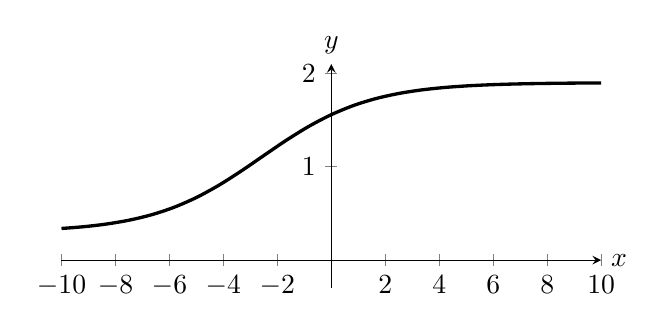
\begin{tikzpicture}
      \begin{axis}[
        clip=false,
        y post scale=0.5,
        domain=-10:10, 
        ytickmin=0,ytickmax=3,
        ytick={1,2},
        xtickmin=-10,xtickmax=10,
        xtick={-10,-8,-6,-4,-2,2,4,6,8,10},
        ymin=-0.3, ymax=2.1,
        xlabel=$x$, ylabel=$y$,
        axis lines=center,
        every axis y label/.style={at=(current axis.above origin),anchor=south},
        every axis x label/.style={at=(current axis.right of origin),anchor=west},
        axis on top,
        ]          
        \addplot [very thick,smooth] {0.3 + 1.6/(1 + exp(-0.5*(x + 2.6))};
      \end{axis}
    \end{tikzpicture}
    \end{image}
  \begin{multipleChoice}
    \choice{As $x$ increases, $f(x)$ is increasing at an increasing rate.}
    \choice[correct]{As $x$ increases, $f(x)$ is increasing at a decreasing rate.}
    \choice{As $x$ increases, $f(x)$ is increasing at a constant rate.}
    \choice{As $x$ increases, $f(x)$ is decreasing at a decreasing rate.}
    \choice{As $x$ increases, $f(x)$ is decreasing at an increasing rate.}
  \end{multipleChoice}
\end{problem}
\end{document}
